%\documentclass[hyperref={pdfpagelabels=false},slidetop,9pt]{beamer}
\documentclass[slidetop,8pt]{beamer}
\usepackage[T1]{fontenc}
\usepackage[utf8]{inputenc}
\newcommand{\id}{71}
\newcommand{\nom}{Théorie des mécanismes}
\newcommand{\sequence}{04}
\newcommand{\nomsequence}{Liaisons entre les solides}
\newcommand{\num}{02}
\newcommand{\type}{KH}
\newcommand{\descrip}{Liaisons équivalentes, hyperstatisme, liaisons en série et en parallèle, théorie des graphes}
\newcommand{\competences}{B2-12: Proposer une modélisation des liaisons avec leurs caractéristiques géométriques. \\ &  B2-13: Proposer un modèle cinématique paramétré à partir d'un système réel, d'une maquette numérique ou d'u \\ &  B2-17: Simplifier un modèle de mécanisme. \\ &  B2-18: Modifier un modèle pour le rendre isostatique. \\ &  C1-04: Proposer une démarche permettant d'obtenir une loi entrée-sortie géométrique.  \\ &  C2-05: Caractériser le mouvement d'un repère par rapport à un autre repère. \\ &  C2-06: Déterminer les relations entre les grandeurs géométriques ou cinématiques. }
\newcommand{\nbcomp}{7}
\newcommand{\systemes}{}
\newcommand{\systemesnum}{}
\newcommand{\systemessansaccent}{}
\newcommand{\ilot}{2}
\newcommand{\ilotstr}{02}
\newcommand{\dossierilot}{\detokenize{Ilot_02 }}

\usepackage{etex}
\usepackage{tikz}
\usepackage[european]{circuitikz}
\usepackage{pgf}
\usepackage[all]{xy}
\usepackage{pgfpages}
\usepackage{graphbox}
\usepackage{pdfpages}
%\usepackage[adobe-utopia]{mathdesign}
\usepackage{ifthen}
\usepackage{cancel}
\usepackage{framed}
\usepackage{subfig}
\usepackage{tabularx}
\usepackage{setspace}
\usepackage{soul}
\usepackage{schemabloc}
\usepackage{eqnarray}
\usepackage[dot, phantomtext]{dashundergaps}
\usepackage{media9}
\usepackage{multimedia}
\usepackage{textcomp}
\usefonttheme[onlymath]{serif}

\author{Renaud Costadoat}
\institute{Lycée Dorian}

\usepackage{multido}
\usepackage{multirow}
\usepackage{multicol} % Portions de texte en colonnes
\usepackage{flafter}%floatants après la référence

\usepackage{color}
\usepackage{xcolor}
\usepackage{colortbl}

\usepackage[gen]{eurosym}
\usepackage{tikz}
%\usepackage{pstricks,pst-node,pst-tree,pst-solides3d}
\usepackage{lmodern}
\usepackage[francais]{babel}
\usepackage{pslatex}
\usetheme{renaud}
\usepackage{times}
\usepackage[frenchmath]{newtxsf} % for sans serif symbols
\renewcommand{\familydefault}{\sfdefault}
%\usepackage{amsfonts}
%\usepackage{amsmath}
%\usepackage{mathastext}
\usepackage{verbatim}
\usepackage{moreverb}
%\usetikzlibrary{arrows,shapes}
\usepackage{graphicx}
\usepackage{psfrag}
\usepackage{wrapfig}
\usepackage{etoolbox}

\definecolor{gris25}{gray}{0.75}
\definecolor{bleu}{RGB}{18,33,98}
\definecolor{bleuf}{RGB}{42,94,171}
\definecolor{bleuc}{RGB}{231,239,247}
\definecolor{rougef}{RGB}{185,18,27}
\definecolor{rougec}{RGB}{255,188,204}%255,230,231
\definecolor{vertf}{RGB}{103,126,82}
\definecolor{vertc}{RGB}{220,255,191}

\setlength\parindent{24pt}
\parskip 7.2pt
\parindent 8pt

\newenvironment{rem}[1][\hsize]%
{%
    \def\FrameCommand
   {%
\rotatebox{90}{\textit{\textsf{Remarque}}} 
       {\color{bleuf}\vrule width 3pt}%
       \hspace{0pt}%must no space.
       \fboxsep=\FrameSep\colorbox{bleuc}%
  }%
    \MakeFramed{\hsize#1\advance\hsize-\width\FrameRestore}%
}%
{\endMakeFramed}%


\newenvironment{savoir}[1][\hsize]%
{%
    \def\FrameCommand
    {%
\rotatebox{90}{\textit{\textsf{Savoir}}} 
        {\color{bleuf}\vrule width 3pt}%
        \hspace{0pt}%must no space.
        \fboxsep=\FrameSep\colorbox{bleuc}%
    }%
    \MakeFramed{\hsize#1\advance\hsize-\width\FrameRestore}%
}%
{\endMakeFramed}%

\newenvironment{prob}[1][\hsize]%
{%
    \def\FrameCommand%
    {%
\rotatebox{90}{\textit{\textsf{Problematique}}} 
        {\color{rougef}\vrule width 3pt}%
        \hspace{0pt}%must no space.
        \fboxsep=\FrameSep\colorbox{rougec}%
    }%
    \MakeFramed{\hsize#1\advance\hsize-\width\FrameRestore}%
}%
{\endMakeFramed}%

\newenvironment{obj}[1][\hsize]%
{%
    \def\FrameCommand%
    {%
\rotatebox{90}{\textit{\textsf{Objectif}}} 
        {\color{vertf}\vrule width 3pt}%
        \hspace{0pt}%must no space.
        \fboxsep=\FrameSep\colorbox{vertc}%
    }%
    \MakeFramed{\hsize#1\advance\hsize-\width\FrameRestore}%
}%
{\endMakeFramed}%

\newenvironment{defi}[1][\hsize]%
{%
    \def\FrameCommand%
    {%
\rotatebox{90}{\textit{\textsf{Definition}}} 
        {\color{bleuf}\vrule width 3pt}%
        \hspace{0pt}%must no space.
        \fboxsep=\FrameSep\colorbox{rougec}%
    }%
    \MakeFramed{\hsize#1\advance\hsize-\width\FrameRestore}%
}%
{\endMakeFramed}%


\newenvironment{hypo}[1][\hsize]%
{%
    \def\FrameCommand%
    {%
\rotatebox{90}{\textit{\textsf{Hypothèse\\}}} 
        {\color{bleuf}\vrule width 3pt}%
        \hspace{0pt}%must no space.
        \fboxsep=\FrameSep\colorbox{bleuc}%
    }%
    \MakeFramed{\hsize#1\advance\hsize-\width\FrameRestore}%
}%
{\endMakeFramed}%


\newenvironment{prop}[1][\hsize]%
{%
    \def\FrameCommand%
    {%
\rotatebox{90}{\textit{\textsf{Propriété}}} 
        {\color{bleuf}\vrule width 3pt}%
        \hspace{0pt}%must no space.
        \fboxsep=\FrameSep\colorbox{bleuc}%
    }%
    \MakeFramed{\hsize#1\advance\hsize-\width\FrameRestore}%
}%
{\endMakeFramed}%

\newenvironment{props}[1][\hsize]%
{%
    \def\FrameCommand%
    {%
\rotatebox{90}{\textit{\textsf{Propriétés}}} 
        {\color{bleuf}\vrule width 3pt}%
        \hspace{0pt}%must no space.
        \fboxsep=\FrameSep\colorbox{bleuc}%
    }%
    \MakeFramed{\hsize#1\advance\hsize-\width\FrameRestore}%
}%
{\endMakeFramed}%

\newenvironment{exemple}[1][\hsize]%
{%
    \def\FrameCommand%
    {%
\rotatebox{90}{\textit{\textsf{Exemple}}} 
        {\color{vertf}\vrule width 3pt}%
        \hspace{0pt}%must no space.
        \fboxsep=\FrameSep\colorbox{vertc}%
    }%
    \MakeFramed{\hsize#1\advance\hsize-\width\FrameRestore}%
}%
{\endMakeFramed}%

\newenvironment{resultat}[1][\hsize]%
{%
    \def\FrameCommand%
    {%
\rotatebox{90}{\textit{\textsf{Résultat}}} 
        {\color{rougef}\vrule width 3pt}%
%        {\color{bleuf}\vrule width 3pt}%
        \hspace{0pt}%must no space.
        \fboxsep=\FrameSep\colorbox{rougec}%
    }%
    \MakeFramed{\hsize#1\advance\hsize-\width\FrameRestore}%
}%
{\endMakeFramed}%

\newenvironment{methode}[1][\hsize]%
{%
    \def\FrameCommand%
    {%
\rotatebox{90}{\textit{\textsf{Méthode\\}}} 
        {\color{rougef}\vrule width 3pt}%
        \hspace{0pt}%must no space.
        \fboxsep=\FrameSep\colorbox{rougec}%
    }%
    \MakeFramed{\hsize#1\advance\hsize-\width\FrameRestore}%
}%
{\endMakeFramed}%

\newenvironment{theo}[1][\hsize]%
{%
    \def\FrameCommand%
    {%
\rotatebox{90}{\textit{\textsf{Théorème\\}}} 
        {\color{rougef}\vrule width 3pt}%
        \hspace{0pt}%must no space.
        \fboxsep=\FrameSep\colorbox{rougec}%
    }%
    \MakeFramed{\hsize#1\advance\hsize-\width\FrameRestore}%
}%
{\endMakeFramed}%

\newenvironment{warn}[1][\hsize]%
{%
    \def\FrameCommand%
    {%
\rotatebox{90}{\textit{\textsf{Attention\\}}} 
        {\color{rougef}\vrule width 3pt}%
        \hspace{0pt}%must no space.
        \fboxsep=\FrameSep\colorbox{rougec}%
    }%
    \MakeFramed{\hsize#1\advance\hsize-\width\FrameRestore}%
}%
{\endMakeFramed}%

% \usepackage{pstricks}
%\usepackage{minitoc}
% \setcounter{minitocdepth}{4}

\setcounter{tocdepth}{2}

% \mtcselectlanguage{french} 

%\usepackage{draftcopy}% "Brouillon"
% \usepackage{floatflt}
\usepackage{psfrag}
%\usepackage{listings} % Permet d'insérer du code de programmation
\renewcommand{\baselinestretch}{1.2}

% Changer la num�rotation des figures :
% ------------------------------------
% \makeatletter
% \renewcommand{\thefigure}{\ifnum \c@section>\z@ \thesection.\fi
%  \@arabic\c@figure}
% \@addtoreset{figure}{section}
% \makeatother
 


%%%%%%%%%%%%
% Définition des vecteurs %
%%%%%%%%%%%%
 \newcommand{\vect}[1]{\overrightarrow{#1}}

%%%%%%%%%%%%
% Définition des torseusr %
%%%%%%%%%%%%

 \newcommand{\torseur}[1]{%
\left\{{#1}\right\}
}

\newcommand{\torseurcin}[3]{%
\left\{\mathcal{#1} \left(#2/#3 \right) \right\}
}

\newcommand{\torseurstat}[3]{%
\left\{\mathcal{#1} \left(#2\rightarrow #3 \right) \right\}
}

 \newcommand{\torseurc}[8]{%
%\left\{#1 \right\}=
\left\{
{#1}
\right\}
 = 
\left\{%
\begin{array}{cc}%
{#2} & {#5}\\%
{#3} & {#6}\\%
{#4} & {#7}\\%
\end{array}%
\right\}_{#8}%
}

 \newcommand{\torseurcol}[7]{
\left\{%
\begin{array}{cc}%
{#1} & {#4}\\%
{#2} & {#5}\\%
{#3} & {#6}\\%
\end{array}%
\right\}_{#7}%
}

 \newcommand{\torseurl}[3]{%
%\left\{\mathcal{#1}\right\}_{#2}=%
\left\{%
\begin{array}{l}%
{#1} \\%
{#2} %
\end{array}%
\right\}_{#3}%
}

 \newcommand{\vectv}[3]{%
\vect{V\left( {#1} \in {#2}/{#3}\right)}
}


\newcommand{\vectf}[2]{%
\vect{R\left( {#1} \rightarrow {#2}\right)}
}

\newcommand{\vectm}[3]{%
\vect{\mathcal{M}\left( {#1}, {#2} \rightarrow {#3}\right)}
}


 \newcommand{\vectg}[3]{%
\vect{\Gamma \left( {#1} \in {#2}/{#3}\right)}
}

 \newcommand{\vecto}[2]{%
\vect{\Omega\left( {#1}/{#2}\right)}
}

\newcommand{\reponse}[1][4]
{
\multido{}{#1}
{
\begin{center}
\makebox[0.9\linewidth]{\dotfill} \end{center}
}}


% }$$\left\{\mathcal{#1} \right\}_{#2} =%
% \left\{%
% \begin{array}{c}%
%  #3 \\%
%  #4 %
% \end{array}%
% \right\}_{#5}}


%  ------------------------------------------
% | Modification du formatage des sections : | 
%  ------------------------------------------

% Grands titres :
% ---------------

\newcommand{\titre}[1]{%
\begin{center}
      \bigskip
      \rule{\textwidth}{1pt}
      \par\vspace{0.1cm}
      
      \textbf{\large #1}
      \par\rule{\textwidth}{1pt}
    \end{center}
    \bigskip
  }

% Supprime le numéro du chapitre dans la numérotation des sections:
% -----------------------------------------------------------------
\makeatletter
\renewcommand{\thesection}{\@arabic\c@section}
\makeatother


% \titleformat{\chapter}[display]
% {\normalfont\Large\filcenter}
% {}
% {1pc}
% {\titlerule[1pt]
%   \vspace{1pc}%
%   \Huge}[\vspace{1ex}%
% \titlerule]


%%%% Chapitres Comme PY Pechard %%%%%%%%%
% numéro du chapitre
\DeclareFixedFont{\chapnumfont}{OT1}{phv}{b}{n}{80pt}
% pour le mot " Chapitre "
\DeclareFixedFont{\chapchapfont}{OT1}{phv}{m}{it}{40pt}
% pour le titre
\DeclareFixedFont{\chaptitfont}{T1}{phv}{b}{n}{25pt}

\definecolor{gris}{gray}{0.75}
\setbeamertemplate{section in toc}[sections numbered]

\newlength{\RoundedBoxWidth}
\newsavebox{\GrayRoundedBox}
\newenvironment{GrayBox}[1][\dimexpr\textwidth-4.5ex]%
   {\setlength{\RoundedBoxWidth}{\dimexpr#1}
    \begin{lrbox}{\GrayRoundedBox}
       \begin{minipage}{\RoundedBoxWidth}}%
   {   \end{minipage}
    \end{lrbox}
    \begin{center}
    \begin{tikzpicture}%
       \draw node[draw=bleuf,fill=bleuc,rounded corners,%
             inner sep=2ex,text width=\RoundedBoxWidth]%
             {\usebox{\GrayRoundedBox}};
    \end{tikzpicture}
    \end{center}}
    
\ifdef{\prive}{\pgfpagesuselayout{2 on 1}[a4paper,border shrink=0mm]}
\ifdef{\prive}{\setbeamertemplate{navigation symbols}{}}
\setbeamertemplate{itemize item}[ball]
%\setbeamertemplate{blocks}[rounded]%[shadow=true]
\setbeamercolor{block title}{fg=white,bg=grisf}        % titre block normal 
\setbeamercolor{block body}{fg=grisf,bg=grisc!50}      % corps block normal
\setbeamercolor{block body alerted}{fg=white,bg=warning}   % idem pour un block alerte

\title{\nom}
\date{S\sequence \ - \type\num}

\begin{document}
\shorthandoff{:!}
\bibliographystyle{abbrvnat-fr}

\usebackgroundtemplate%
{%
    \centering
\includegraphics[width=\paperwidth]{/home/renaud/Documents/Renaud/GitHub/Sciences-Ingenieur/img/fond2}%
}

{
\setbeamertemplate{navigation symbols}{}
\setbeamertemplate{headline}[pagetitre]
\setbeamertemplate{footline}[pagetitre]
\usebackgroundtemplate{\centering
\includegraphics[width=\paperwidth]{/home/renaud/Documents/Renaud/GitHub/Sciences-Ingenieur/img/fond}}
\frame{\titlepage}
}



\section{Les liaisons élémentaires}

{\frame{
\frametitle{Les liaisons mécaniques}

\begin{obj}
\begin{itemize}
 \item Le principal outil utilisé afin de modéliser le comportement d'un mécanisme est le torseur car il permet d'exprimer n'importe quel \textbf{champ de vecteurs}.
 \item La mécanique appliquée au Sciences Industrielles a décomposé le mouvement général d'un solide afin de proposer des mouvements de base pour lesquels il est possible de spécifier la forme d'un torseur.
\end{itemize}
\end{obj}
}}


{\frame{
\frametitle{Les liaisons élémentaires}

\begin{defi}
Une liaison élémentaire entre deux solides $S_1$ et $S_2$ est obtenue à partir du contact d'une surface géométrique élémentaire liée à $S_1$ sur une surface géométrique élémentaire liée à $S_2$.
\end{defi}

\vfill

\begin{center}
\renewcommand{\arraystretch}{2}
\begin{tabular}{|c|c|c|c|}
\hline
 & Plan & Cylindre & Sphère \\
\hline
Sphère & \begin{minipage}{0.1\linewidth}
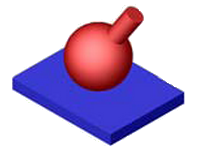
\includegraphics[width=\linewidth]{img/11}
\end{minipage} & \begin{minipage}[c]{0.1\linewidth}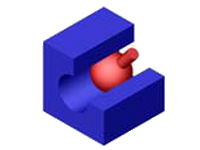
\includegraphics[width=\linewidth]{img/12}\end{minipage} & \begin{minipage}{0.1\linewidth}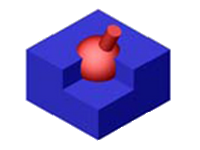
\includegraphics[width=\linewidth]{img/13}\end{minipage} \\
\hline
Cylindre & \begin{minipage}{0.1\linewidth}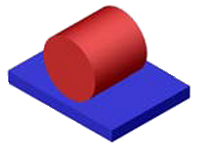
\includegraphics[width=\linewidth]{img/21}\end{minipage} & \begin{minipage}{0.1\linewidth}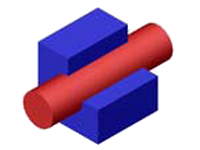
\includegraphics[width=\linewidth]{img/22}\end{minipage} &   \\
\hline
Plan & \begin{minipage}{0.1\linewidth}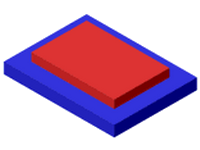
\includegraphics[width=\linewidth]{img/31}\end{minipage} & & \\
\hline
\end{tabular}
\end{center}
}}

{\frame{
\frametitle{Les liaisons composées}

Une liaison composée est obtenue par association cohérente de liaisons élémentaires.


\begin{center}
\renewcommand{\arraystretch}{2}
\begin{tabular}{|c|c|c|c|}
\hline
Glissière & \begin{minipage}{0.1\linewidth}
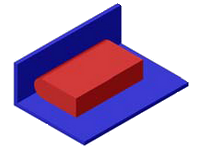
\includegraphics[width=\linewidth]{img/221}
\end{minipage} & \begin{minipage}[c]{0.1\linewidth}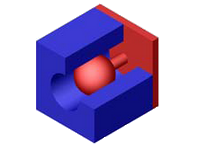
\includegraphics[width=\linewidth]{img/212}\end{minipage} & Pivot \\
\hline
Encastrement & \begin{minipage}{0.1\linewidth}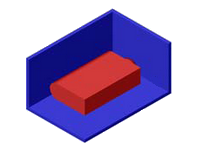
\includegraphics[width=\linewidth]{img/211}\end{minipage} & \begin{minipage}{0.1\linewidth}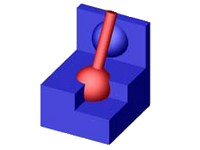
\includegraphics[width=\linewidth]{img/222}\end{minipage} & Sphérique à doigt  \\
\hline
\end{tabular}
\end{center}

\vfill

Liaison avec surface hélicoïdale

\begin{center}
\begin{tabular}{|c|c|}
\hline
\renewcommand{\arraystretch}{0.1}
 & \\
\renewcommand{\arraystretch}{3}
Hélicoïdale & \begin{minipage}{0.1\linewidth}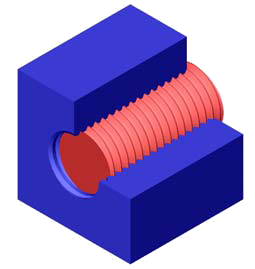
\includegraphics[width=\linewidth]{img/03}\end{minipage} \\
\renewcommand{\arraystretch}{0.1}
 & \\
\hline
\end{tabular}
\end{center}
}}

{\frame{
\frametitle{Degrés de liberté ou de mobilité d'une liaison}

\begin{itemize}
 \item Les \textbf{degrés de liberté} d'une liaison entre deux solides $S_1$ et $S_2$ correspondent aux mouvements relatifs indépendants autorisés au sein de cette liaison entre $S_1$ et $S_2$.

 \item Il existe 6 mouvements élémentaires possibles d'un solide dans l'espace rapporté à un repère $R(\overrightarrow{x},\overrightarrow{y},\overrightarrow{z})$

\begin{itemize}
 \item 3 translations : $T_x$, $T_y$, $T_z$,
 \item 3 rotations : $R_x$, $R_y$, $R_z$.
\end{itemize}

 \item \textbf{m} est le nombre de degrés de liberté d'une liaison

 \item Le degré de liaison d'une liaison vaut, dans l'espace, \textbf{6-m}, c'est le \textbf{complémentaire} du degré de liberté.

 \item Dans le plan $(A,\overrightarrow{x},\overrightarrow{y})$, les 3 mouvements possibles d'un solide sont :
\begin{itemize}
 \item 2 translations : $T_x$, $T_y$,
 \item 1 rotation : $R_z$.
\end{itemize}

Le degré de liaison d'une liaison vaut, dans le plan, \textbf{3-m}.
\end{itemize}
}}

{\frame{
\frametitle{Les liaisons mécaniques}

\begin{minipage}{0.4\linewidth}
\begin{enumerate}
 \item Liaison pivot,
 \item Liaison glissière,
 \item Liaison pivot glissant,
 \item Liaison hélicoïdale,
 \item Liaison sphérique ou rotule,
 \item Liaison sphérique à doigt,
 \item Liaison appui plan,
 \item Liaison linéaire annulaire,
 \item Liaison linéaire rectiligne,
 \item Liaison ponctuelle,
 \item Liaison encastrement.
\end{enumerate}
\end{minipage}
\hfill
\begin{minipage}{0.55\linewidth}
\begin{defi}
Caractéristiques des liaisons parfaites:
\begin{itemize}
 \item des contacts sans frottement entre les surfaces,
 \item des surfaces de contact géométriquement parfaites,
 \item aucun jeu.
\end{itemize}
\end{defi}
\end{minipage}
}}


{\frame{
\frametitle{Liaison pivot}

\begin{itemize}
 \item Deux solides $S_1$ et $S_2$ sont en liaison pivot si, au cours du fonctionnement, le seul mouvement relatif possible est une rotation autour d'un axe,
 \item \ifdef{\public}{Degré de liberté: $R_1=1$, degré de liberté égal à 1.}{}
\end{itemize}

\vfill

\begin{minipage}{0.35\linewidth}
 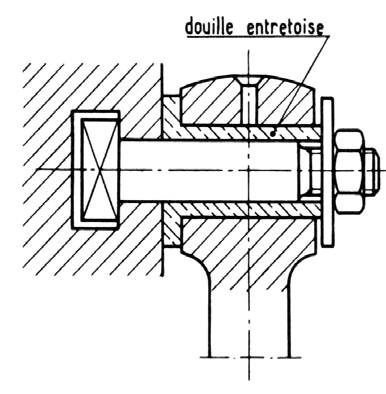
\includegraphics[width=\linewidth]{img/pivot_des}
\end{minipage}\hfill
\begin{minipage}{0.6\linewidth}
\begin{tabular}{c c c}
Vue plane de face & Vue plane de côté & Perspective \\
\ifdef{\public}{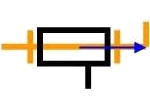
\includegraphics[width=40pt]{img/pivot1} & 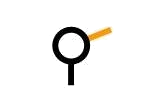
\includegraphics[width=40pt]{img/pivot2} & 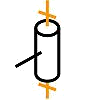
\includegraphics[width=40pt]{img/pivot3}}{}
\end{tabular}
\end{minipage}
}}

{\frame{
\frametitle{Liaison glissière}

\begin{itemize}
 \item Deux solides $S_1$ et $S_2$ sont en liaison glissière si, au cours du fonctionnement, le seul mouvement relatif possible est une translation le long d'un axe,
 \item \ifdef{\public}{Degré de liberté: $T_1=1$, degré de liberté égal à 1}{}
\end{itemize}

\vfill

\begin{minipage}{0.35\linewidth}
 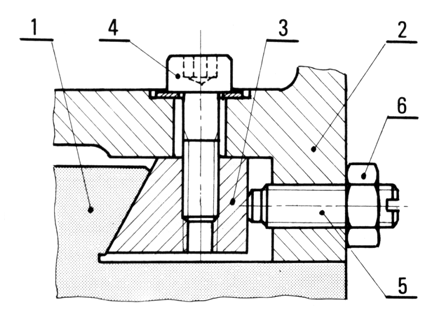
\includegraphics[width=\linewidth]{img/gliss_des}
\end{minipage}\hfill
\begin{minipage}{0.6\linewidth}
\begin{tabular}{c c c}
Vue plane de face & Vue plane de côté & Perspective \\
\ifdef{\public}{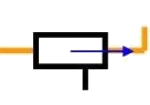
\includegraphics[width=40pt]{img/gliss1} & 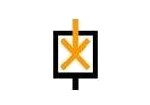
\includegraphics[width=40pt]{img/gliss2} & 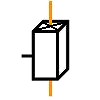
\includegraphics[width=40pt]{img/gliss3}}{}
\end{tabular}
\end{minipage}
}}

{\frame{
\frametitle{Liaison pivot glissant}

\begin{itemize}
 \item Deux solides $S_1$ et $S_2$ sont en liaison pivot glissant si, au cours du fonctionnement, le seul mouvement relatif possible résulte d'une rotation et d'une translation par rapport à un axe,
 \item \ifdef{\public}{Degré de liberté: $T_1=1$ et $R_1=1$, degré de liberté égal à 2.}{}
\end{itemize}

\vfill

\begin{minipage}{0.35\linewidth}
 \centering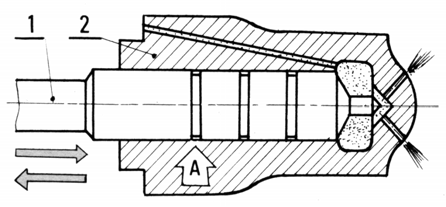
\includegraphics[width=0.8\linewidth]{img/pivgliss_des}
\end{minipage}\hfill
\begin{minipage}{0.6\linewidth}
\begin{tabular}{c c c}
Vue plane de face & Vue plane de côté & Perspective \\
\ifdef{\public}{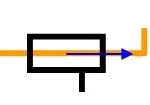
\includegraphics[width=40pt]{img/pivgliss1} & 
\includegraphics[width=40pt]{img/pivgliss2} & 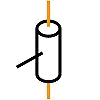
\includegraphics[width=40pt]{img/pivgliss3}}{}
\end{tabular}
\end{minipage}
}}

{\frame{
\frametitle{Liaison hélicoïdale}

\begin{itemize}
 \item Deux solides $S_1$ et $S_2$ sont en liaison hélicoïdale si, au cours du fonctionnement, le seul mouvement relatif possible résulte d'une rotation et d'une translation proportionnelles par rapport à un axe,
 \item \ifdef{\public}{Degré de liberté: $T_1$ et $R_1$ sont dépendants. Si $k$ est le pas, on a $k\times \theta_1 = 2\pi \times \Delta_1$ , degré de liberté égal à 1.}{}
\end{itemize}

\vfill

\begin{minipage}{0.35\linewidth}
 \centering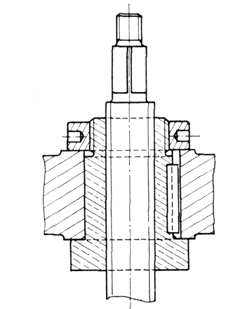
\includegraphics[width=0.8\linewidth]{img/heli_des}
\end{minipage}\hfill
\begin{minipage}{0.6\linewidth}
\begin{tabular}{c c c}
Vue plane de face & Vue plane de côté & Perspective \\
\ifdef{\public}{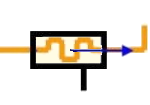
\includegraphics[width=40pt]{img/heli1} & 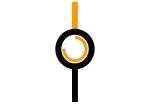
\includegraphics[width=40pt]{img/heli2} & 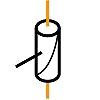
\includegraphics[width=40pt]{img/heli3}}{}
\end{tabular}
\end{minipage}
}}

{\frame{
\frametitle{Liaison rotule}

\begin{itemize}
 \item Deux solides $S_1$ et $S_2$ sont en liaison sphérique ou rotule si, au cours du fonctionnement, le seul mouvement relatif possible est une rotation autour d'un point,
 \item \ifdef{\public}{Degré de liberté: $R_1=1$, $R_2=1$ et $R_3=1$, degré de liberté égal à 3.}{}
\end{itemize}

\vfill

\begin{minipage}{0.35\linewidth}
 \centering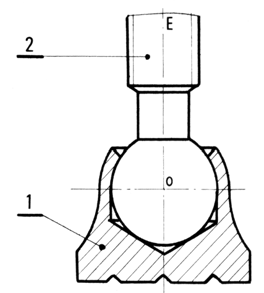
\includegraphics[width=0.8\linewidth]{img/rot_des}
\end{minipage}\hfill
\begin{minipage}{0.6\linewidth}
\begin{tabular}{c c c}
Vue plane de face & Vue plane de côté & Perspective \\
\ifdef{\public}{ & 
\includegraphics[width=40pt]{img/rot1} & }{}
\end{tabular}
\end{minipage}
}}

{\frame{
\frametitle{Liaison sphérique à doigt}

\begin{itemize}
 \item Deux solides $S_1$ et $S_2$ sont en liaison sphérique à doigt si, au cours du fonctionnement, le seul mouvement relatif possible résulte de la rotation par rapport à deux axes concourants,
 \item \ifdef{\public}{Degré de liberté: $R_1=1$ et $R_2=1$, degré de liberté égal à 2.}{}
\end{itemize}

\vfill
\begin{minipage}{0.35\linewidth}
 \centering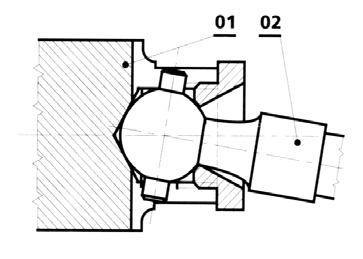
\includegraphics[width=0.8\linewidth]{img/sphdoi_des}
\end{minipage}\hfill
\begin{minipage}{0.6\linewidth}
\begin{tabular}{c c c}
Vue plane de face & Vue plane de côté & Perspective \\
\ifdef{\public}{ & 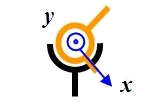
\includegraphics[width=40pt]{img/sphdoi1} & }{}
\end{tabular}
\end{minipage}
}}

{\frame{
\frametitle{Liaison appui plan}

\begin{itemize}
 \item Deux solides $S_1$ et $S_2$ sont en liaison appui plan si, au cours du fonctionnement, le seul mouvement relatif possible résulte d'une rotation autour d'un axe et de la translation le long de deux axes perpendiculaires au premier,
 \item \ifdef{\public}{Degré de liberté: $R_1=1$, $T_2=1$ et $T_3=1$, degré de liberté égal à 3.}{}
\end{itemize}

\vfill

\begin{minipage}{0.35\linewidth}
 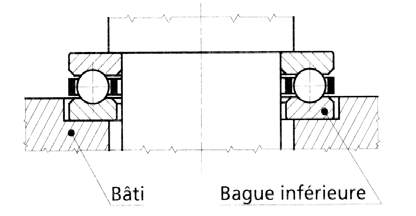
\includegraphics[width=\linewidth]{img/plan_des}
\end{minipage}\hfill
\begin{minipage}{0.6\linewidth}
\begin{tabular}{c c c}
Vue plane de face & Vue plane de côté & Perspective \\
\ifdef{\public}{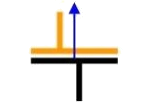
\includegraphics[width=40pt]{img/plan1} & 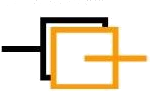
\includegraphics[width=40pt]{img/plan2} & 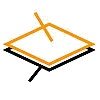
\includegraphics[width=40pt]{img/plan3}}{}
\end{tabular}
\end{minipage}
}}

{\frame{
\frametitle{Liaison linéaire annulaire}

\begin{itemize}
 \item Deux solides $S_1$ et $S_2$ sont en liaison linéaire annulaire si, au cours du fonctionnement, le seul mouvement relatif possible résulte d'une rotation autour d'un point et d'une translation suivant un axe passant par ce point,
 \item \ifdef{\public}{Degré de liberté: $T_1=1$, $R_1=1$, $R_2=1$ et $R_3=1$, degré de liberté égal à 4.}{}
\end{itemize}

\vfill

\begin{minipage}{0.35\linewidth}
 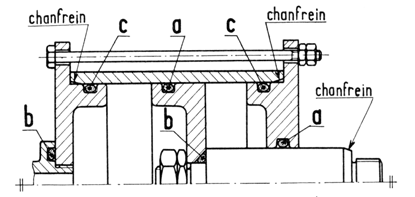
\includegraphics[width=\linewidth]{img/linan_des}
\end{minipage}\hfill
\begin{minipage}{0.6\linewidth}
\begin{tabular}{c c c}
Vue plane de face & Vue plane de côté & Perspective \\
\ifdef{\public}{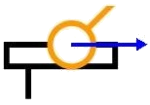
\includegraphics[width=40pt]{img/linan1} & 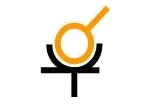
\includegraphics[width=40pt]{img/linan2} & 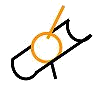
\includegraphics[width=40pt]{img/linan3}}{}
\end{tabular}
\end{minipage}
}}

{\frame{
\frametitle{Liaison linéaire rectiligne}

\begin{itemize}
 \item Deux solides $S_1$ et $S_2$ sont en liaison linéaire rectiligne si, au cours du fonctionnement, le seul mouvement relatif possible résulte d'une rotation autour de deux axes et de la translation le long de deux autres axes, l'une des rotations et l'une des translations étant relatives au même axe,
  \item \ifdef{\public}{Degré de liberté: $T_2=1$, $T_3=1$, $R_1=1$ et $R_2=1$, degré de liberté égal à 4.}{}
\end{itemize}

\vfill

\begin{minipage}{0.35\linewidth}
 \centering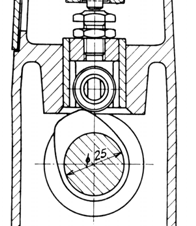
\includegraphics[width=.7\linewidth]{img/linrec_des}
\end{minipage}\hfill
\begin{minipage}{0.6\linewidth}
\begin{tabular}{c c c}
Vue plane de face & Vue plane de côté & Perspective \\
\ifdef{\public}{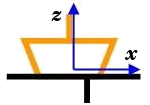
\includegraphics[width=40pt]{img/linrec1} & 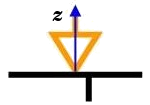
\includegraphics[width=40pt]{img/linrec2} & 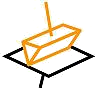
\includegraphics[width=40pt]{img/linrec3}}{}
\end{tabular}
\end{minipage}
}}

{\frame{
\frametitle{Liaison ponctuelle}

\begin{itemize}
 \item Deux solides $S_1$ et $S_2$ sont en liaison ponctuelle si, au cours du fonctionnement, le seul mouvement relatif possible résulte de la rotation autour d'un point et de la translation le long de deux axes concourants en ce point
 \item \ifdef{\public}{Degré de liberté: $T_2=T_3=1$ et $R_1=R_2=R_3=1$, degré de liberté égal à 5.}{}
\end{itemize}

\vfill

\begin{minipage}{0.35\linewidth}
 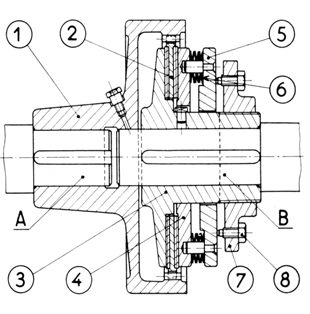
\includegraphics[width=0.9\linewidth]{img/pon_des}
\end{minipage}\hfill
\begin{minipage}{0.6\linewidth}
\begin{tabular}{c c c}
Vue plane de face & Vue plane de côté & Perspective \\
\ifdef{\public}{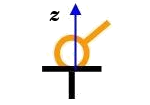
\includegraphics[width=40pt]{img/pon1} & 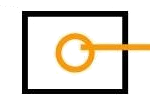
\includegraphics[width=40pt]{img/pon2} & 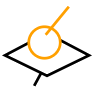
\includegraphics[width=40pt]{img/pon3}}{}
\end{tabular}
\end{minipage}
}}

{\frame{
\frametitle{Liaison encastrement}

\begin{itemize}
 \item Deux solides $S_1$ et $S_2$ sont en liaison encastrement s'il n'existe aucun degré de liberté entre les solides,
 \item \ifdef{\public}{Degré de liberté: $T_x=T_y=T_z=R_x=R_y=R_z=0$, degré de liberté nul.}{}
\end{itemize}

\vfill

\begin{minipage}{0.35\linewidth}
 \centering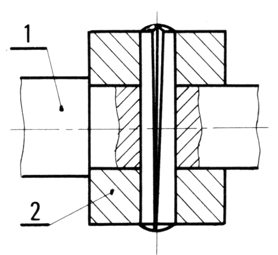
\includegraphics[width=0.8\linewidth]{img/enc_des}
\end{minipage}\hfill
\begin{minipage}{0.6\linewidth}
\begin{tabular}{c c c}
Vue plane de face & Vue plane de côté & Perspective \\
\ifdef{\public}{ & \includegraphics[width=40pt]{img/enc1} & }{}
\end{tabular}
\end{minipage}
}}

\section{Torseur cinématique}

{\frame{
\frametitle{Torseur cinématique}

\begin{itemize}
 \item Le torseur cinématique est le torseur représentant le champ de vecteurs vitesse d'un solide S dans le repère R. 
\begin{itemize}
 \item Sa résultante est le vecteur vitesse de rotation du solide : $\overrightarrow{\Omega_{S/R}}$,
 \item Son moment en un point P est le vecteur vitesse linéaire du point P : $\overrightarrow{V_{P\in {S/R}}}$,
\end{itemize}
Le Torseur cinématique du solide S par rapport à R s'écrit:
\begin{center}
\ifdef{\public}{$\left\{V_{S/R}\right\}=\left\{ \begin{array}{c} \overrightarrow{\Omega_{S/R}} \\ \overrightarrow{V_{P\in {S/R}}} \end{array}\right\}_{P}=\left\{ \begin{array}{cc} \omega_x & V_x \\ \omega_y & V_y \\ \omega_z & V_z \end{array}\right\}_{P}$}{\vspace{30pt}}
\end{center}
\item Et on peut écrire ce torseur en un point quelconque du solide pour en obtenir sa vitesse en utilisant le théorème de Varignon. 
\end{itemize}
}}

{\frame{
\frametitle{Exemples de torseurs cinématiques}

\begin{itemize}
 \item Dans un mouvement de translation, $\overrightarrow{\Omega_{S/R}}$ est nul, donc le torseur devient un torseur couple :
\begin{center}
$\left\{V_{S/R}\right\}_{P}=\left\{ \begin{array}{c} \overrightarrow{0} \\ \overrightarrow{V_{P\in {S/R}}} \end{array}\right\}_{P}$
\end{center}
 \item $\overrightarrow{V_{P\in S/R}}=\overrightarrow{0}$ si le point P appartient à l'axe de rotation du solide. Si on exprime le torseur au point P : 
\begin{center}
$\left\{V_{S/R}\right\}_{P}=\left\{ \begin{array}{c} \overrightarrow{\Omega_{S/R}} \\ \overrightarrow{0} \end{array}\right\}_{P}$
\end{center}
\textit{Attention}: Ce torseur à un moment non-nul si on l'exprime en un point qui n'appartient pas à l'axe de rotation du solide
\end{itemize}
}}

{\frame{
\frametitle{Exemples de torseurs cinématiques}
\begin{itemize}
 \item Un mouvement hélicoïdal est caractérisé par une rotation combinée à une translation, l'axe de rotation étant confondu avec la direction de la translation. Cela entraine que pour tout point A de l'axe de rotation, $\overrightarrow{V_{A\in {S/R}}}$ est colinéaire à $\overrightarrow{\Omega_{S/R}}$. Le torseur cinématique de S en A appartenant à l'axe de rotation s'écrit de la façon suivante :

\begin{center}
$\left\{V_{S/R}\right\}_{A}=\left\{ \begin{array}{c} \overrightarrow{\Omega_{S/R}} \\ \overrightarrow{V_{A\in {S/R}}} \end{array}\right\}_{A}$, avec $\overrightarrow{V_{A\in {S/R}}}=\lambda.\overrightarrow{\Omega_{S/R}}$
\end{center}
\vfill
 \item Pour tous autres points P du solide, le vecteur vitesse est une combinaison de $\overrightarrow{V_{A\in {S/R}}}$ et du terme $\overrightarrow{\Omega_{S/R}}\wedge \overrightarrow{AP}$
\end{itemize}
}}

{\frame{
\frametitle{Torseurs cinématiques classiques}

Les torseurs classiques sont définis en connaissant les mouvements autorisés et les degrés de liberté de la liaison.

\begin{center}
\begin{tabular}{|m{3cm}|c|m{3cm}|}
\hline
Liaison pivot & Torseur cinématique & Axes nécessaires \\
\ifdef{\public}{ & $\left\{ \begin{array}{cc} \omega_x & 0 \\ 0 & 0 \\ 0 & 0 \end{array}\right\}_{O}$  & 1 axe $(O,\overrightarrow{x})$}{ &  & \\ &  & \\ &  &} \\
\hline
Liaison glissière & Torseur cinématique & Axes nécessaires \\
\ifdef{\public}{ & $\left\{ \begin{array}{cc} 0 & V_x \\ 0 & 0 \\ 0 & 0 \end{array}\right\}_{O}$  & 1 direction $\overrightarrow{x}$}{ &  & \\ &  & \\ &  &} \\
\hline
Liaison pivot glissant & Torseur cinématique & Axes nécessaires \\
\ifdef{\public}{ & $\left\{ \begin{array}{cc} \omega_x & V_x \\ 0 & 0 \\ 0 & 0 \end{array}\right\}_{O}$  & 1 axe $(O,\overrightarrow{x})$ }{ &  & \\ &  & \\ &  &} \\
\hline
\end{tabular}
\end{center}
}}

{\frame{
\frametitle{Torseurs cinématiques classiques}

\begin{center}
\begin{tabular}{|m{3cm}|c|m{3cm}|}
\hline
Liaison hélicoïdale & Torseur cinématique & Axes nécessaires \\
\ifdef{\public}{ & $\left\{ \begin{array}{cc} \omega_x & V_x \\ 0 & 0 \\ 0 & 0 \end{array}\right\}_{O}$  & \begin{tabular}{l} 1 axe $(O,\overrightarrow{x})$ \\ $V_x=\frac{p.\omega_x}{2\pi}$ \end{tabular} }{ &  & \\ &  & \\ &  &} \\
\hline
Liaison sphérique ou rotule & Torseur cinématique & Axes nécessaires \\
\ifdef{\public}{ & $\left\{ \begin{array}{cc} \omega_x & 0 \\ \omega_y & 0 \\ \omega_z & 0 \end{array}\right\}_{O}$  & 0 axe }{ &  & \\ &  & \\ &  &}  \\
\hline
Liaison sphérique à doigts & Torseur cinématique & Axes nécessaires \\
\ifdef{\public}{ & $\left\{ \begin{array}{cc} \omega_x & 0 \\ \omega_y & 0 \\ 0 & 0 \end{array}\right\}_{O}$  & 2 axes, $(O,\overrightarrow{x})$, $(O,\overrightarrow{y})$  }{ &  & \\ &  & \\ &  &} \\
\hline
Liaison appui plan & Torseur cinématique & Axes nécessaires \\
\ifdef{\public}{ & $\left\{ \begin{array}{cc} 0 & V_x \\ 0 & V_y \\ \omega_z & 0 \end{array}\right\}_{O}$  & \begin{tabular}{l} 1 axe $(O,\overrightarrow{z})$ \\ normale au plan \end{tabular} }{ &  & \\ &  & \\ &  &}  \\
\hline
\end{tabular}
\end{center}
}}

{\frame{
\frametitle{Torseurs cinématiques classiques}

\begin{center}
\begin{tabular}{|m{3cm}|c|m{3cm}|}
\hline
Liaison linéaire annulaire & Torseur cinématique & Axes nécessaires \\
\ifdef{\public}{ & $\left\{ \begin{array}{cc} \omega_x & V_x \\ \omega_y & 0 \\ \omega_z & 0 \end{array}\right\}_{O}$  & 1 axe $(O,\overrightarrow{x})$ }{ &  & \\ &  & \\ &  &}\\
\hline
Liaison linéaire rectiligne & Torseur cinématique & Axes nécessaires \\
\ifdef{\public}{ & $\left\{ \begin{array}{cc} \omega_x & V_x \\ 0 & V_y \\ \omega_z & 0 \end{array}\right\}_{O}$  & \begin{tabular}{l} 2 axes $(O,\overrightarrow{x})$, $(O,\overrightarrow{z})$ \\ direction de la ligne $\overrightarrow{x}$ \\ normale au plan $\overrightarrow{z}$ \end{tabular} }{ &  & \\ &  & \\ &  &} \\
\hline
Liaison ponctuelle & Torseur cinématique & Axes nécessaires \\
\ifdef{\public}{ & $\left\{ \begin{array}{cc} \omega_x & V_x \\ \omega_y & V_y \\ \omega_z & 0 \end{array}\right\}_{O}$  & \begin{tabular}{l} 1 axe $(O,\overrightarrow{z})$ \\ normale au plan \end{tabular} }{ &  & \\ &  & \\ &  &} \\
\hline
Liaison encastrement & Torseur cinématique & Axes nécessaires \\
\ifdef{\public}{ & $\left\{ \begin{array}{cc} 0 & 0 \\ 0 & 0 \\ 0 & 0 \end{array}\right\}_{O}$  & 0 axe }{ &  & \\ &  & \\ &  &} \\
\hline
\end{tabular}
\end{center}
}}

\section{Torseur actions mécaniques}

{\frame{
\frametitle{Torseur d'actions mécaniques transmissibles}

L'action mécanique du solide $(S_1)$ sur $(S_2)$ au niveau de la liaison $l_i$ peut être définie par un torseur :
\begin{center}
  \begin{math}
	\left\{T_{i(S_2\rightarrow S_1)}\right\}=\left\{ \begin{array}{c} \overrightarrow{R_{(S_2\rightarrow S_1)}} \\ \overrightarrow{M_{O,(S_2\rightarrow S_1)}}\end{array}\right\}_O
  \end{math}
\end{center}

avec :
\begin{center}
  \begin{math}
\begin{array}{l} \overrightarrow{R_{(S_2\rightarrow S_1)}}=X_i.\overrightarrow{x}+Y_i.\overrightarrow{y}+Z_i.\overrightarrow{z} \\ \overrightarrow{M_{O,(S_2\rightarrow S_1)}}=L_i.\overrightarrow{x}+M_i.\overrightarrow{y}+N_i.\overrightarrow{z}\end{array}
  \end{math}
\end{center}


Le torseur d'actions mécaniques peut s'écrire ainsi :
\begin{center}
  \begin{math}
	\left\{T_{i(S_2\rightarrow S_1)}\right\}=\left\{ \begin{array}{cc} X_i & L_i \\ Y_i & M_i \\ Z_i & N_i \end{array}\right\}_O
  \end{math}
\end{center}


Les composantes $X_i$, $Y_i$, $Z_i$, $L_i$, $M_i$, $N_i$ non nulles sont les \textbf{inconnues statiques} de la liaison $l_i$.

$n_{si}$ est le nombre d'inconnues statiques indépendantes.
}}

{\frame{
\frametitle{Torseurs d'actions transmissibles classiques}

Les torseurs classiques sont définis en connaissant les mouvements autorisés et les degrés de liberté de la liaison.

\begin{center}
\begin{tabular}{|m{3cm}|c|m{3cm}|}
\hline
Liaison pivot & Torseur d'actions transmissibles & Axes nécessaires \\
\ifdef{\public}{ & $\left\{ \begin{array}{cc} X & 0 \\ Y & M \\ Z & N \end{array}\right\}_{O}$  & 1 axe $(O,\overrightarrow{x})$}{ &  & \\ &  & \\ &  &} \\
\hline
Liaison glissière & Torseur d'actions transmissibles & Axes nécessaires \\
\ifdef{\public}{ & $\left\{ \begin{array}{cc} 0 & L \\ Y & M \\ Z & N \end{array}\right\}_{O}$  & 1 direction $\overrightarrow{x}$}{ &  & \\ &  & \\ &  &} \\
\hline
Liaison pivot glissant & Torseur d'actions transmissibles & Axes nécessaires \\
\ifdef{\public}{ & $\left\{ \begin{array}{cc} 0 & 0 \\ Y & M \\ Z & N \end{array}\right\}_{O}$  & 1 axe $(O,\overrightarrow{x})$ }{ &  & \\ &  & \\ &  &} \\
\hline
\end{tabular}
\end{center}
}}

{\frame{
\frametitle{Torseurs d'actions transmissibles classiques}

\begin{center}
\begin{tabular}{|m{3cm}|c|m{3cm}|}
\hline
Liaison hélicoïdale & Torseur d'actions transmissibles & Axes nécessaires \\
\ifdef{\public}{ & $\left\{ \begin{array}{cc} X & L \\ Y & M \\ Z & N \end{array}\right\}_{O}$  & \begin{tabular}{l} 1 axe $(O,\overrightarrow{x})$ \\ $L=\frac{p.X}{2\pi}$ \end{tabular} }{ &  & \\ &  & \\ &  &} \\
\hline
Liaison sphérique ou rotule & Torseur d'actions transmissibles & Axes nécessaires \\
\ifdef{\public}{ & $\left\{ \begin{array}{cc} X & 0 \\ Y & 0 \\ Z & 0 \end{array}\right\}_{O}$  & 0 axe }{ &  & \\ &  & \\ &  &}  \\
\hline
Liaison sphérique à doigts & Torseur d'actions transmissibles & Axes nécessaires \\
\ifdef{\public}{ & $\left\{ \begin{array}{cc} X & 0 \\ Y & 0 \\ Z & N \end{array}\right\}_{O}$  & 2 axes, $(O,\overrightarrow{x})$, $(O,\overrightarrow{y})$  }{ &  & \\ &  & \\ &  &} \\
\hline
\end{tabular}
\end{center}
}}

{\frame{
\frametitle{Torseurs d'actions transmissibles classiques}

\begin{center}
\begin{tabular}{|m{3cm}|c|m{3cm}|}
\hline
Liaison appui plan & Torseur d'actions transmissibles & Axes nécessaires \\
\ifdef{\public}{ & $\left\{ \begin{array}{cc} 0 & L \\ 0 & M \\ Z & 0 \end{array}\right\}_{O}$  & \begin{tabular}{l} 1 axe $(O,\overrightarrow{z})$ \\ normale au plan \end{tabular} }{ &  & \\ &  & \\ &  &}  \\
\hline
Liaison linéaire annulaire & Torseur d'actions transmissibles & Axes nécessaires \\
\ifdef{\public}{ & $\left\{ \begin{array}{cc} 0 & 0 \\ Y & 0 \\ Z & 0 \end{array}\right\}_{O}$  & 1 axe $(O,\overrightarrow{x})$ }{ &  & \\ &  & \\ &  &}\\
\hline
Liaison linéaire rectiligne & Torseur d'actions transmissibles & Axes nécessaires \\
\ifdef{\public}{ & $\left\{ \begin{array}{cc} 0 & 0 \\ 0 & M \\ Z & 0 \end{array}\right\}_{O}$  & \begin{tabular}{l} 2 axes $(O,\overrightarrow{x})$, $(O,\overrightarrow{z})$ \\ direction de la ligne $\overrightarrow{x}$ \\ normale au plan $\overrightarrow{z}$ \end{tabular} }{ &  & \\ &  & \\ &  &} \\
\hline
\end{tabular}
\end{center}
}}

{\frame{
\frametitle{Torseurs d'actions transmissibles classiques}

\begin{center}
\begin{tabular}{|m{3cm}|c|m{3cm}|}
\hline
Liaison ponctuelle & Torseur d'actions transmissibles & Axes nécessaires \\
\ifdef{\public}{ & $\left\{ \begin{array}{cc} 0 & 0 \\ 0 & 0 \\ Z & 0 \end{array}\right\}_{O}$  & \begin{tabular}{l} $(O,\overrightarrow{z})$ \\ normale au plan \end{tabular} }{ &  & \\ &  & \\ &  &} \\
\hline
Liaison encastrement & Torseur d'actions transmissibles & Axes nécessaires \\
\ifdef{\public}{ & $\left\{ \begin{array}{cc} X & L \\ Y & M \\ Z & N \end{array}\right\}_{O}$  & 0 axe }{ &  & \\ &  & \\ &  &} \\
\hline
\end{tabular}
\end{center}
}}


{\frame{
\frametitle{Liaison parfaite}

Une liaison parfaite lorsque le produit de ses torseurs cinématique et statique est nul. Ces torseurs sont dit \textbf{réciproques}.

Soit:
  \begin{math}
	\left\{T_{i(S_2\rightarrow S_1)}\right\}\times\left\{V_{i(S_2/S_1)}\right\}=0
  \end{math}

D'où, 
  \begin{math}
\overrightarrow{M_{O,(S_2\rightarrow S_1)}}.\overrightarrow{\Omega_{i(S_2/S_1)}}+\overrightarrow{R_{(S_2\rightarrow S_1)}}.\overrightarrow{V_{i(O\in S_2/S_1)}}=0
  \end{math}

Donc,
  \begin{math}
	L_i.\alpha_i+M_i.\beta_i+N_i.\gamma_i+X_i.u_i+Y_i.v_i+Z_i.w_i=0
  \end{math}

Ainsi, $n_{ci}+n_{si}=6$

Pour une liaison pivot: $n_{si}=5$

\begin{center}
  \begin{math}
	\left\{T_{i(S_2\rightarrow S_1)}\right\}=\left\{ \begin{array}{cc} X_i & 0 \\ Y_i & M_i \\ Z_i & N_i \end{array}\right\}_O
	\left\{V_{i(S_2/S_1)}\right\}=\left\{ \begin{array}{cc} \alpha_i & 0 \\ 0 & 0 \\ 0 & 0 \end{array}\right\}_O
  \end{math}
\end{center}
}}

\section{Schématisation}

{\frame{
\frametitle{La schématisation}

\begin{itemize}
 \item La \textbf{représentation} des liaisons vue précédemment permet de définir des \textbf{schémas} qui permettent de représenter \textbf{une partie de la géométrie} du mécanisme.
 \item La géométrie représentée constitue le strict minimum nécessaire à la modélisation du mécanisme pour une application donnée.
\end{itemize}

\vfill

\begin{exemple}
\begin{itemize}
 \item Pour une étude cinématique, l'épaisseur d'une pièce n'a aucune importance, pas plus que le moyen technologique utilisé pour réaliser un encastrement,
 \item Ces informations ne doivent, par conséquent, pas être représentées.
\end{itemize}
\end{exemple}
}}

{\frame{
\frametitle{Schéma cinématique}

\begin{center}
 \includegraphics[width=0.6\linewidth]{img/meule1}
\end{center}

\begin{itemize}
 \item Il représente les mouvements relatifs entre sous-ensembles cinématiques.
 \item Il fait l'objet de la norme NF EN 23-952.
 \item Seules les mobilités sont modélisées (pas la réalisation des liaisons)
\end{itemize}
}}

{\frame{
\frametitle{Les éléments du schéma cinématique}

Les liaisons normalisées et les engrenages...

\begin{center}
 %\ifdef{\public}{\includegraphics[width=0.8\linewidth]{img/tableau {\includegraphics[width=0.8\linewidth]{img/tableau_vide}}
 \includegraphics[width=0.8\linewidth]{img/tableau}
\end{center}
}}

{\frame{
\frametitle{Les éléments du schéma cinématique}

... les engrenages et les liens flexibles

\begin{center}
 %\ifdef{\public}{\includegraphics[width=0.8\linewidth]{img/tableau2}}{\includegraphics[width=0.8\linewidth]{img/tableau2_vide}}
 \includegraphics[width=0.8\linewidth]{img/tableau2}
\end{center}
}}

{\frame{
\frametitle{Schéma architectural}
\begin{center}
\includegraphics[width=0.8\linewidth]{img/meule2}
\end{center}

\begin{itemize}
 \item Il met en évidence la \textbf{nature} et les \textbf{positions} relatives des différentes \textbf{liaisons élémentaires}
 \item Les \textbf{pièces sans mouvement relatif} ne sont pas \textbf{distinguées} les unes des autres
 \item Ses \textbf{composants} sont les \textbf{constituants} du schéma cinématique
\end{itemize}
}}

{\frame{
\frametitle{Schéma technologique}

\begin{center}
\includegraphics[width=0.7\linewidth]{img/meule3}
\end{center}

\begin{itemize}
 \item Il permet la description de la nature et de l'\textbf{agencement} des principaux \textbf{composants} d'un produit, généralement représentés par des symboles normalisés.
\end{itemize}
}}

{\frame{
\frametitle{Les trois types de schémas}

\begin{center}
\includegraphics[width=\linewidth]{img/meule4}
\end{center}
}}

{\frame{
\frametitle{Pompe à engrenage (Cinématique)}

\begin{minipage}{0.48\linewidth}
 \ifdef{\public}{\centering\includegraphics[width=\linewidth]{img/pompe2}}{\centering\includegraphics[width=\linewidth]{img/pompe1}}
\end{minipage}
\hfill
\begin{minipage}{0.48\linewidth}
 \ifdef{\public}{\centering\includegraphics[width=\linewidth]{img/pompe2_1}}{}
\end{minipage}
}}

{\frame{
\frametitle{Pompe à engrenage (Architecture)}

\begin{minipage}{0.48\linewidth}
 \ifdef{\public}{\centering\includegraphics[width=0.8\linewidth]{img/pompe4}}{\centering\includegraphics[width=0.8\linewidth]{img/pompe3}}
\end{minipage}
\hfill
\begin{minipage}{0.48\linewidth}
 \ifdef{\public}{\centering\includegraphics[width=0.8\linewidth]{img/pompe4_1}}{}
\end{minipage}
}}

{\frame{
\frametitle{Pompe à engrenage (Technologique)}

\begin{minipage}{0.48\linewidth}
 \ifdef{\public}{\centering\includegraphics[width=0.8\linewidth]{img/pompe6}}{\centering\includegraphics[width=0.8\linewidth]{img/pompe5}}
\end{minipage}
\hfill
\begin{minipage}{0.48\linewidth}
 \ifdef{\public}{\centering\includegraphics[width=0.8\linewidth]{img/pompe6_1}}{}
\end{minipage}
}}

{\frame{
\frametitle{Les liaisons d'un mécanisme}

\begin{savoir}
\begin{itemize}
 \item Vous devez être capables de modéliser une liaison à partir des surfaces qui caractérisent le contact entre ses pièces,
 \item Déterminer les degrés de liberté et de liaison de celle-ci,
 \item Écrire le torseur correspondant et l'exprimer en n'importe quel point,
 \item Les schémas cinématiques, architecturaux et technologies sont la base de la communication de la structure d'un mécanisme.
\end{itemize}
\end{savoir}

\begin{obj}
 \begin{itemize}
  \item Représenter la géométrie des pièces plus proche du réel,
  \item Modéliser l'ensemble de l'architecture d'un mécanisme par ses liaisons,
  \item Intégrer le phénomène d'hyperstaticité dans la résolution des boucles fermées.
 \end{itemize}
\end{obj}
}}
\end{document}
